\documentclass[letterpaper,11pt,twoside]{article}
\usepackage[utf8]{inputenc}
\usepackage{amsmath,amsfonts,amssymb,amsthm,latexsym}
\usepackage[spanish,es-noshorthands]{babel}
\usepackage[T1]{fontenc}
\usepackage{lmodern}
\usepackage{graphicx,hyperref}
\usepackage{tikz,pgf}
\usepackage{multicol}
\usepackage{fancyhdr}
\usepackage[height=9.5in,width=7in]{geometry}
\usepackage{fancyhdr}
\pagestyle{fancy}
\fancyhead[LE]{
\includegraphics[height=12pt]{Images/logo-colegio.png} Aritm\`{e}tica $6^{\circ}$}
\fancyhead[RE]{}
\fancyhead[RO]{\textit{Germ\'an Avenda\~no Ram\'irez, Lic. U.D., M.Sc. U.N.}}
\fancyhead[LO]{}

\author{Germ\'an Avenda\~no Ram\'irez, Lic. U.D., M.Sc. U.N.}
\title{\begin{minipage}{.2\textwidth}

\includegraphics[height=1.75cm]{Images/logo-colegio.png}\end{minipage}
\begin{minipage}{.55\textwidth}
\begin{center}
Taller 08, Divisi\`{o}n en $\mathbb{N}$\\
Aritmética $6^{\circ}$
\end{center}
\end{minipage}\hfill
\begin{minipage}{.2\textwidth}

\includegraphics[height=1.75cm]{Images/logo-sed.png} 
\end{minipage}}
\date{}
\thispagestyle{plain}
\begin{document}
\maketitle
Nombre: \hrulefill Curso: \underline{\hspace*{44pt}} Fecha: \underline{\hspace*{2.5cm}}
\begin{multicols}{2}
\section*{Lo que s\`{e}}
Realice la siguiente actividad en el cuaderno:

Manuel compró un terreno, con las dimensiones que se observan en el plano, por un precio de \$ 18'750\,000.
\begin{center}
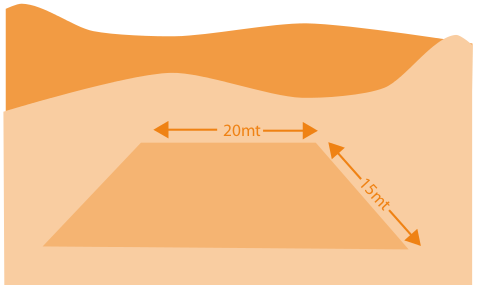
\includegraphics[scale=.5]{Images/terreno.png} 
\end{center}
\begin{itemize}
\item ¿Cuál es el área del terreno?
\item ¿Cuál es el valor de cada metro cuadrado del terreno?
\item ¿Qué operación deben efectuar para resolver la situación propuesta?
\end{itemize}
Para resolver la situación, primero se halla el área del terreno: 300 m$^{2}$. ¿Por qué?

Luego, se puede realizar la siguiente \emph{división de números naturales:}
\begin{center}
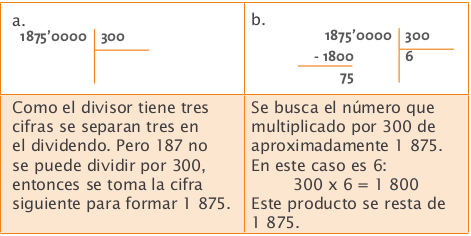
\includegraphics[scale=.5]{Images/division.png} 
\end{center}
\end{multicols}


\end{document}
